% Shared standalone design for the editable figure reconstructions.
\documentclass[tikz,border=5pt,10pt]{standalone}
\usepackage[T1]{fontenc}
\usepackage[utf8]{inputenc}
\usepackage{newpxtext,newpxmath}
\usepackage[scaled=.94]{sourcesanspro}
\usepackage{pgfplots}
\pgfplotsset{compat=1.18}
\usetikzlibrary{arrows.meta,calc,positioning,decorations.pathreplacing,
  decorations.markings,patterns,matrix,shapes.geometric,fit,backgrounds,
  intersections,angles,quotes}
\definecolor{ink}{HTML}{203746}
\definecolor{accent}{HTML}{146C78}
\definecolor{muted}{HTML}{667780}
\definecolor{signalred}{HTML}{B94B44}
\color{ink}
\tikzset{>=Latex,line width=.8pt,
  every node/.style={font=\small},
  axis/.style={->,draw=muted,line width=.5pt},
  guide/.style={draw=muted,dashed,line width=.45pt},
  curve/.style={draw=accent,line width=1pt},
  marker/.style={circle,fill=accent,inner sep=1.5pt},
  labelbox/.style={fill=white,inner sep=2pt}}

\begin{document}
\begin{tikzpicture}[x=1cm,y=1cm]
\draw[axis] (0,0)--(4.8,0) node[right] {$x$};
\draw[curve,domain=0:2.4,samples=91] plot (\x,{2.1*sin(75*\x)^2*(.7+.3*cos(180*\x))});
\foreach \x in {0,.2,...,2.4} {\draw[accent!65] (\x,0)--(\x,{2.1*sin(75*\x)^2*(.7+.3*cos(180*\x))});}
\foreach \x in {2.6,2.8,...,4.4} {\fill[signalred] (\x,0) circle(1.4pt);}
\node[below] at (0,-.1) {$0$};\node[below] at (2.4,-.1) {$1$};\node[below] at (4.4,-.1) {$T=Q/N$};
\draw[decorate,decoration={brace,mirror,amplitude=4pt},signalred] (2.6,-.55)--(4.4,-.55);
\node[signalred,below] at (3.5,-.72) {zeros};
\node at (2.25,2.65) {$f_n^Q=f(n/N)$};
\draw[->] (5.05,1)--node[above] {$\mathcal F_Q$}(6,1);
\begin{scope}[shift={(8.6,0)}]
\draw[axis] (-2.2,0)--(2.3,0) node[right] {$\omega$};
\draw[curve,domain=-2:2,samples=180] plot (\x,{abs(1.85*exp(-3*\x*\x)+.12*exp(-.2*\x*\x)*cos(210*\x))});
\foreach \x in {-2,-1.8,...,2} {\fill[accent] (\x,{abs(1.85*exp(-3*\x*\x)+.12*exp(-.2*\x*\x)*cos(210*\x))}) circle(1pt);}
\node[below] at (-2,-.1) {$-\pi N$};\node[below] at (0,-.1) {$0$};\node[below] at (2,-.1) {$\pi N$};
\node at (0,2.65) {$|\widehat f(\omega)|$};
\node at (0,-.9) {$\Delta\omega=\dfrac{2\pi}{T}$};
\end{scope}
\node at (5.35,-1.8) {$\displaystyle\frac1N\widehat f_k^Q\approx\widehat f(2\pi k/T)$};
\end{tikzpicture}
\end{document}
